%\RequirePackage[2020-02-02]{latexrelease}
\documentclass[a4paper,twoside,12pt]{report}
 %openright
\newcommand{\documenttype}{Report 1}
\newcommand{\thesistitle}{Elektromagnetiske sensorer og digital signalbehandling}
\newcommand{\thesissubtitle}{Metaldetektor}

\newcommand{\thesisauthor}{Gruppe 2} % Your name :) 
\newcommand{\studentnumber}{s111111}
\newcommand{\thedate}{14 May 2022} % For example "June, 2019"

\newcommand{\department}{62739}
\newcommand{\departmentdescriber}{Elektroteknologi}
\newcommand{\addressI}{Brovej, Building 118}
\newcommand{\addressII}{2800 Kgs. Lyngby}
\newcommand{\departmentwebsite}{www.byg.dtu.dk}
%\usepackage{microtype}      % better looking text
\usepackage[table]{xcolor}
\usepackage{fontspec}       % Package for custom fonts
\usepackage[]{geometry}     % Package for changing page margins (before fancyhdr) 
\usepackage{fancyhdr}       % Package to change header and footer
\usepackage{tocloft}
\usepackage{parskip}        % Package to tweak paragraph skipping (instead of indents a small skip is added after every paragraph)
\usepackage{titlesec}
\usepackage{tikz}           % Package for drawing
\usepackage{pgfplots}       % Package for creating graphs and charts
\usepackage{xcolor}         % Package for defining DTU colours to be used

\usepackage{amsmath}        % For aligning equations among other
\usepackage{siunitx}        % SI units

\usepackage{listings}       % Package for inserting code, (before cleveref)
\PassOptionsToPackage{hyphens}{url} % Ability to line break urls at hyphens
\usepackage{hyperref}       % Package for cross referencing (also loads url package)
\usepackage{cleveref}       % improved cross referencing
\usepackage{textcomp}       % \textdegree = °C and other useful symbols
\usepackage{textgreek}
\usepackage[danish]{babel} % localisation 
\usepackage{caption}        % better captions
\usepackage{subcaption}     % for subfigures
%\usepackage{csquotes}       % For biblatex with babel
%\usepackage[backend=biber,style=authoryear,sorting=none]{biblatex} % Package for bibliography (citing)
\bibliography{bibliography.bib}
\usepackage{tabularx}       % for ability to adjust column spacing in tabular better
\usepackage{booktabs}       % for better tables
%\captionsetup[table]{name=Tabel} % for changing the table navn to fx danish.
%\captionsetup[figure]{name=Figur} % for changing the figur navn to fx danish.
\usepackage{float}          % floating figures in correct places
\usepackage{calc}           % Adds ability for latex to calculate (3pt+2pt) 
\usepackage{blindtext}
%\usepackage{contour}
\usepackage[final]{pdfpages}
\usepackage{minted}
\usepackage{subfiles} % Best loaded last in the preamble
\usepackage[export]{adjustbox}
\usepackage{longtable}
\usepackage{pgf-pie}

\usepackage{wrapfig}

\input{Setup/Settings.tex}

\begin{document}

\pagenumbering{roman}
\title{\thesistitle} 
\author{\thesisauthor} 
\date{\thedate} 

\begin{titlepage}

\newgeometry{left=11mm,right=11mm,top=50mm,bottom=0pt}
\pagecolor{frontbackcolor}
\color{\frontpagetextcolour}

%{ % Thesis title (to change see Setup/Settings.tex) 
\Large
%\begin{tabular}{p{\linewidth}}
%\begin{tabular}{p{12000pt}}
\TitleFont{\thesistitle}\\
\large\thesissubtitle \\
\thesisauthor
%\end{tabular}
%}

% DTU department (to change see Setup/Settings.tex) 
\begin{tikzpicture}[remember picture,overlay]
\node[anchor=north east, 
      xshift=-10mm, 
      yshift=-12mm] 
      at (current page.north east) 
      {
        \color{\frontpagetextcolour}
        \begin{tabular}{r} 
        \textbf{\department} \\ 
        \departmentdescriber
        \end{tabular}
      }; 
\end{tikzpicture}

% DTU logo
\begin{tikzpicture}[remember picture,overlay]
\node[anchor=north west, 
      xshift=8.9mm, 
      yshift=-8.3mm] 
     at (current page.north west) 
     {\includegraphics[width=14.75mm,keepaspectratio]{Overleaf/Pictures/Logos/\dtulogocolour_\targetcolourmodel.pdf}}; 
\end{tikzpicture}

% Cover photo
\begin{tikzpicture}[remember picture,overlay]
\node[anchor=south, % anchor is bottom of picture
      xshift=0pt, 
      yshift=100mm] % shifting picture to actually be at the bottom of the page
     at (current page.south) % placement at bottom of the page
     {\includegraphics[width=21cm,keepaspectratio]{Overleaf/Pictures/Frontpage/Metal_detector_from_World_War_1.jpeg}};
\end{tikzpicture}

% Cover photo of us
\begin{figure}[b!]
    \captionsetup[subfigure]{font={sc,color=white}, labelformat=empty}
    \centering
    \vspace{1mm}
    \begin{subfigure}[1]{0.20\linewidth}
    \includegraphics[width=\linewidth]{Overleaf/Pictures/Frontpage/ardrinon nano.jpg}
    \captionsetup{justification=centering}
    \caption[]{{\small xxxnavnxxx}\\{insæt std}}
    \end{subfigure}
    \hspace{2em}
    \begin{subfigure}[1]{0.20\linewidth}
    \includegraphics[width=\linewidth]{Overleaf/Pictures/Frontpage/ardrinon nano.jpg}
    \captionsetup{justification=centering}
    \caption[]{{\small xxxnavnxxx}\\{insæt std}}
    \end{subfigure}
    \hspace{2em}
    \begin{subfigure}[1]{0.20\linewidth}
    \includegraphics[width=\linewidth]{Overleaf/Pictures/Frontpage/ardrinon nano.jpg}
    \captionsetup{justification=centering}
    \caption[]{{\small xxxnavnxxx}\\{insæt std}}
    \end{subfigure}
    \hspace{2em}
     \begin{subfigure}[1]{0.20\linewidth}
    \includegraphics[width=\linewidth]{Overleaf/Pictures/Frontpage/ardrinon nano.jpg}
    \captionsetup{justification=centering}
    \caption[]{{\small xxxnavnxxx}\\{insæt std}}
    \end{subfigure}
    \hspace{2em}
     \begin{subfigure}[1]{0.20\linewidth}
    \includegraphics[width=\linewidth]{Overleaf/Pictures/Frontpage/ardrinon nano.jpg}
    \captionsetup{justification=centering}
    \caption[]{{\small xxxnavnxxx}\\{insæt std}}
    \end{subfigure}
    \hspace{2em}
     \begin{subfigure}[1]{0.20\linewidth}
    \includegraphics[width=\linewidth]{Overleaf/Pictures/Frontpage/ardrinon nano.jpg}
    \captionsetup{justification=centering}
    \caption[]{{\small xxxnavnxxx}\\{insæt std}}
    \end{subfigure}
    \hspace{2em}
    \vspace{20mm}
\end{figure}
\end{titlepage}
\pagecolor{white}
\newgeometry{top=2.70cm, bottom=2.70cm, outer=2.5cm, inner=2.5cm}
\pagestyle{plain}
\clearpage
\renewcommand{\contentsname}{Indholdsfortegnelse} %This is the name of the content / Indholdsfortegnelse. Changing this will change it in the rapport.
\renewcommand{\figurename}{Figur}
\renewcommand\tablename{Tabel}
\tableofcontents
\clearpage

%%%%%%%%%%%%%%%%%%%%%%%%%%%%%%%%%%%%%%%%%%%%%%%%%%%%%%%
\pagenumbering{arabic}
\subfile{Chapters/01_Introduktion}
\clearpage
\subfile{Chapters/02_Analyse}
\clearpage
\subfile{Chapters/03_Design}
\clearpage
\subfile{Chapters/04_Implementering}
\clearpage
\subfile{Chapters/05_Test}
\clearpage
\subfile{Chapters/06_Konklusion}
\clearpage
%\subfile{Chapters/08_Colours}
%\clearpage
%\subfile{Chapters/09_eksempler}
%\clearpage
%\subfile{Chapters/10_Examples}
%%%%%%%%%%%%%%%%%%%%%%%%%%%%%%%%%%%%%%%%%%%%%%%%%%%%%%%

%\printbibliography[heading=bibintoc,title={Bibliography}]
\clearpage
\appendix
\chapter{Appendiks}
\section{Planlægning}

\subsection{Gantt-skema}
\renewcommand{\arraystretch}{1.5}
\resizebox{\textwidth}{!}{%
    \begin{tabular}{|l|m{0.035\textwidth}|m{0.035\textwidth}|m{0.035\textwidth}|m{0.035\textwidth}|m{0.035\textwidth}||m{0.035\textwidth}|m{0.035\textwidth}|m{0.035\textwidth}|m{0.035\textwidth}|m{0.035\textwidth}||m{0.035\textwidth}|m{0.035\textwidth}|m{0.035\textwidth}|m{0.035\textwidth}|m{0.035\textwidth}|m{0.035\textwidth}|m{0.035\textwidth}|m{0.035\textwidth}|m{0.035\textwidth}|m{0.035\textwidth}|}
\hline
\rowcolor[HTML]{C0C0C0}
Januar      & 2 & 3 & 4 & 5 & 6 & 9 & 10 & 11 & 12 & 13 & 16 & 17 & 18 & 19 & 20 & 21 & 22 \\ \hline
Research    & \cellcolor{black} & \cellcolor{black} & \cellcolor{black} & \cellcolor{black} &                 \cellcolor{black} & & & & & & & & & & & & \\ \hline
Beregninger & \cellcolor{black}&\cellcolor{black} &\cellcolor{black} & & & & & & & & & & & & & & \\ \hline
3D-print    & & &\cellcolor{black} &\cellcolor{black} & & &\cellcolor{black} & & & & & &\cellcolor{black} &\cellcolor{black} & & & \\ \hline
TX PA       & & &\cellcolor{black} &\cellcolor{black} & \cellcolor{black}& \cellcolor{black}& & & & & & & & & & & \\ \hline
RX AMP      & & & & & &\cellcolor{black} &\cellcolor{black} & \cellcolor{black}& \cellcolor{black}& & & & & & & & \\ \hline
Kode        & &\cellcolor{black} &\cellcolor{black} & \cellcolor{black}&\cellcolor{black} &\cellcolor{black} &\cellcolor{black} &\cellcolor{black} & & & & & & & & & \\ \hline
PCB         & & & & & & & & & &\cellcolor{black} &\cellcolor{black} &\cellcolor{black} &\cellcolor{black} & & & & \\ \hline
Tests       & & & & & &\cellcolor{black} & & &\cellcolor{black} & & & & &\cellcolor{black} & & & \\ \hline
PowerPoint  & & & & & & & & & & & & & & \cellcolor{black} & & & \\ \hline
Rapport     & & & & & \cellcolor{black} & \cellcolor{black} & \cellcolor{black} & \cellcolor{black} & \cellcolor{black} & \cellcolor{black} & \cellcolor{black} & \cellcolor{black} & \cellcolor{black} & \cellcolor{black} & \cellcolor{black} & \cellcolor{black} & \cellcolor{black}\\ \hline
    \end{tabular}}

\subsection{Tidsforbrug/fokusområde}
\begin{figure}[!h]
    \centering
    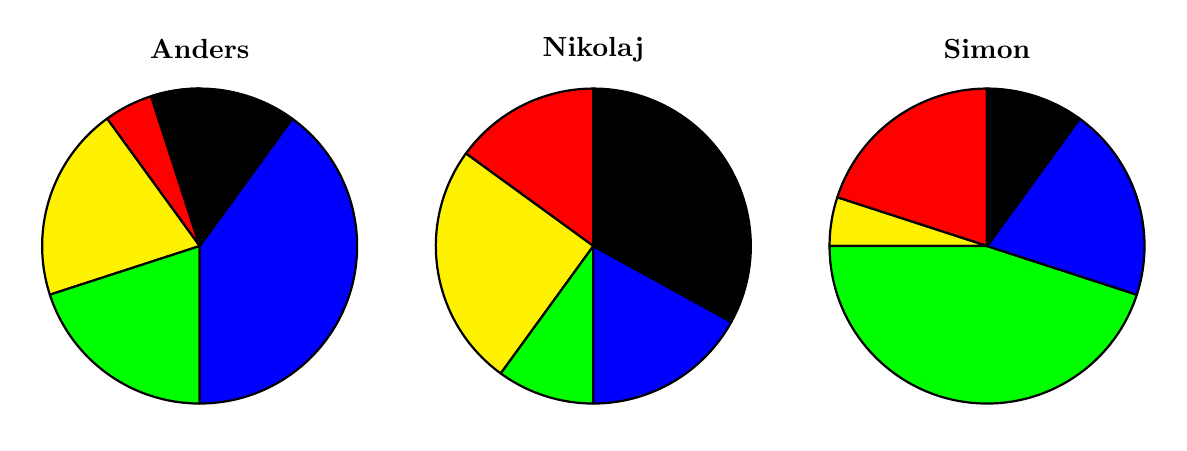
\begin{tikzpicture}
        \pie[radius = 2,                            %Anders
             hide number,
             rotate =90,
             color={red, yellow, green,blue,black}]
                 {10/{}, 20/{}, 20/{}, 40/{}, 15/{}}    %percent
        \pie[pos={5,0},                             %Nikolaj
             radius = 2,
             hide number,
             rotate = 90,
             color={red,yellow,green,blue,black}]
             {15/{}, 25/{}, 10/{}, 17/{}, 33/{}} %percent
        \pie[pos={10,0},                            %Simon
             radius = 2,
             hide number,
             rotate = 90,
             color={red,yellow,green,blue,black}]
             {20/{},5/{},45/{},20/{},10/{}}    %percent
        \node at (0,2.5)    {\textbf{Anders}};
        \node at (5,2.5)    {\textbf{Nikolaj}};
        \node at (10,2.5)   {\textbf{Simon}};
    \end{tikzpicture}
\end{figure}

\noindent\fbox{%
    \parbox{3cm}{%
    \fcolorbox{black}{red}{\phantom{X}}     Research    \\
    \fcolorbox{black}{yellow}{\phantom{X}}  Produktion  \\
    \fcolorbox{black}{green}{\phantom{X}}   Software    \\
    \fcolorbox{black}{blue}{\phantom{X}}    Hardware    \\
    \fcolorbox{black}{black}{\phantom{X}}   Rapport
    }%
}

\clearpage
\section{Beregninger} \label{Chap:Beregninger}

\subsection{Transmitterspole/TX-spole}\vspace{5mm}
\underline{Anvendte konstanter}
\begin{align*}
    \mu_0  &= 1.25663706212 \cdot 10^{-6}\: \frac{H}{m}\\
    \rho_{Cu} &= 1.68 \cdot 10^{-8}\: \Omega \cdot m
\end{align*}

\underline{Valgte parametre}
\begin{align*}
    f_r &= 2.00 kHz\\
    r_{spole} &= 13.7cm\\
    A_{pk-pk} &= 8.00V
\end{align*}

\underline{Approksimation af sinusbølgens amplitude}
$$\boxed{a_n=2\cdot\frac{A}{n\cdot\pi}\cdot sin\left(\frac{n\cdot\pi}{2}\right)}$$
\begin{align*}
    a_1 &= 2\cdot\frac{8V}{\pi}\cdot sin\left(\frac{\pi}{2}\right) &= 5.09V\\
    a_{RMS} &= \frac{a_1}{\sqrt{2}} &= 3.60V
\end{align*}
Da kredsløbet udelukkende er resistivt ved resonans:
$$\;\quad R = \frac{a_{RMS}}{I} = \frac{3.60V}{250mA} \;\; \qquad \qquad \qquad = 14.4\Omega$$

\underline{Transmitterspolens antal vindinger}
$$\boxed{N_{TX}=\frac{R \cdot r_{wire}^2}{2 \cdot r_{coil} \cdot \rho}}$$
Ud fra de tilgængelige kobberledninger ($\rho = \rho_{Cu}$), vælges diameteren 0.355mm.
$$N_{TX} = \frac{14.4\Omega\cdot(\frac{0.355mm}{2})^2}{2 \cdot 13.7cm \cdot 1.68 \cdot 10^{-8}\:\Omega\cdot m} = 98.57 \approx 99$$
\underline{Valg af antal lag}\\
For at spolen og dermed spolehovedet ikke skal blive for højt vælges at spolen skal ligge i 5 lag ($n_{lag}=5$)\vspace{5mm}\\
\underline{Vidden af vindingerne (max)}
    $$\boxed{A_{vidde_{max}}= \left\lceil \frac{N_{TX}}{n_{lag}} \right\rceil \cdot d_{wire}}$$
\begin{align*}
    A_{vidde_{max}}&= \left\lceil \frac{99}{5} \right\rceil \cdot 0.355mm &\\
    &= \;\quad 20 \cdot 0.355mm &= 7.10mm
\end{align*}



\underline{Selvinduktans}
$$\boxed{L[\mu H] = \frac{0.394\cdot r_{spole}^2[cm]\cdot N_{TX}^2}{9\cdot r_{spole}[cm]+10\cdot A_{vidde}[cm]}}$$
$$ L_{TX} = \frac{0.394 \cdot 13.7^2 \cdot 99^2}{9 \cdot 13.7 + 10 \cdot 0.710}\mu H = 5.56mH$$
\underline{Kondensatorens kapacitans}
$$\boxed{f_r= \frac{1}{2\cdot\pi\cdot\sqrt{L \cdot C}} \Leftrightarrow C = \frac{1}{4\cdot\pi^2\cdot f_r^2\cdot L}}$$
$$C = \frac{1}{4\cdot \pi^2\cdot 2kHz\cdot 5.56mH} =1.14\mu F$$

\underline{B-felt}
$$\boxed{\lvert \overrightarrow{B} \rvert = \frac{\mu_0\cdot I\cdot N_{TX}}{2\cdot r_{spole}}}$$
$$\lvert \overrightarrow{B} \rvert = \frac{1.26\cdot10^{-6}\frac{H}{m}\cdot250mA\cdot 99}{2\cdot 13.7cm} = 113.5\mu T$$

\subsection{Modtagerspolen (RX)}
Kravspecifikationens pkt. 16 angiver min. 10mH selvinduktans for modtagerspolen.\\
Ved at angive en selvinduktans, der er dobbelt så stor som kravet, opnås en stor fejlmargin ved eventuelle afvigelser mellem teoretiske udregninger og virkelige forhold.
Med udgangspunkt i dette og med antagelsen af at modtagerspolen får samme vidde som transmitterspolen fås følgende:
\begin{align*}
    L_{RX} &= \frac{0.394\cdot 13.7^2\cdot N_{RX}^2}{9\cdot13.7+10\cdot0.71}\mu H & &=20000\mu H\\
           &= \frac{73.98\cdot N_{RX}^2}{130.43} \mu H                            & &=20000\mu H\\
    \lvert N_{RX} \rvert &= 187.8                                                 & &\approx 188
\end{align*}

\subsection{Modtagerspolen (RX)}
\begin{align*}
    L_{RX} &= \frac{0.394\cdot 13.7^2\cdot N_{RX}^2}{9\cdot13.7+10\cdot0.71}\mu H & &=20000\mu H\\
           &= \frac{73.98\cdot N_{RX}^2}{130.43} \mu H                            & &=20000\mu H\\
    \lvert N_{RX} \rvert &= 187.8                                                 & &\approx 188
\end{align*}
\clearpage
\section{Figurer}
\subsection{PV-diagrammer}

    \begin{figure}[H]
    \includegraphics[width=\textwidth]{Dokumentation/Figures/PV_Buck_MPPT.png}
    \caption{Forskellige itterationer af switch-opsætninger til buck convertere.}
    \end{figure}

    \begin{figure}[H]
    \includegraphics[width=\textwidth]{Dokumentation/Figures/PV_Buck_x-5V.png}
    \caption{Forskellige itterationer af switch-opsætninger til buck convertere.}
    \end{figure}

    \begin{figure}[H]
    \includegraphics[width=\textwidth]{Dokumentation/Figures/PV_Converter switches.png}
    \caption{Forskellige itterationer af switch-opsætninger til buck convertere.}
    \end{figure}

    \begin{figure}[H]
    \includegraphics[width=\textwidth]{Dokumentation/Figures/PV_strøm-spændingsmåler.png}
    \caption{Forskellige itterationer af switch-opsætninger til buck convertere.}
    \end{figure}

\clearpage
\section{VHDL-kode}
%%\lstinputlisting[language=VHDL]{Files/VHDL/xxx.vhd}
\clearpage
\end{document}